\documentclass[paper]{aiaaNew}

%\usepackage[notref,notcite]{showkeys}


\newenvironment{proof}
{}{}


%\documentstyle[10pt,draft,fancyheadings]{AIAAtran}
%\documentstyle[9pt,twocolumn,technote,twoside]{AIAAtran}


\SubmitName{Schaub}

% for conference paper:

\PaperNumber{xxx}

\CoverFigure{}

\Conference{{\bfseries AIAA Guidance, Navigation and \\ Control 
Conference} \\
            August 10--12,~1998 / Boston, MA}

% for a journal simulation cover page:

\JournalName{Journal of Guidance, Navigation and Control}
\JournalIssue{Volume~xx, Number~xx, Jan.--Feb., 2001, Pages xx--xx}

% journal article simulation:

\ArticleIssue{Vol.~24, No.~1, Jan.--Feb., 2001}% first page
\ArticleHeader{Schaub Et Al: New Penalty Functions}% subsequent pages

% journal note simulation:

\NoteHeader{J.Guidance, Vol.~20, No.~13: Engineering Notes}

% set copyright and other notices to appear
% as a footnote at the bottom of the first page:

%\PaperNotice{\CopyrightB{1998}{Hanspeter Schaub}}

\JournalNotice{Presented as Paper~06--3792 at the AIAA
               Guidance, Navigation and Control Conference, San 
Diego,~CA,
               July~29--31,~1996.
               \CopyrightB{1996}{the authors}}

% load the title, author, and abstract for use with the \maketitle command

\title{Title Goes Here}
                                
\author{
%
John J. Doe%
%
  \thanks{Assistant Professor,  
  Aerospace and Ocean Engineering Department.  Senior Member of AIAA.}
  \\
  \emph{\normalsize Virginia Tech, Blacksburg, VA 24061-0203}
}

\abstract{
Abstract should be around 200--300 words.  Explain briefly what the problem is, how does the presented work contribute.  Summarize the paper results
}


\begin{document}


\maketitle




\section{Introduction}
\PARstart{T}{ext}   
goes here.   As seen in Figure~\ref{fig:sample}.  

\begin{itemize}
	\item Explain to reader the general problem discusses in this paper.  Explain the general problem to be investigated, and also show why this is important through examples.  Reference other work or examples, if possible.    
	\item Provide a brief literature review where you outline the previous efforts and works in this area. 
	\item Discuss what the paper will cover.  \emph{Don't discuss results in the introduction.}  
	\item Put your new work in perspective to the previous work in this area.  This helps the reader to understand what all is novel here, and what is taken from other works.  
\end{itemize}


 \subsection{Testing of a Subsection}
 
 text here text here text here text here text here text here text here text here text here text here text here text here text here text here text here text here text here text here text here text here text here text here text here 
 
 \begin{figure}[htb]
 	\centering
 	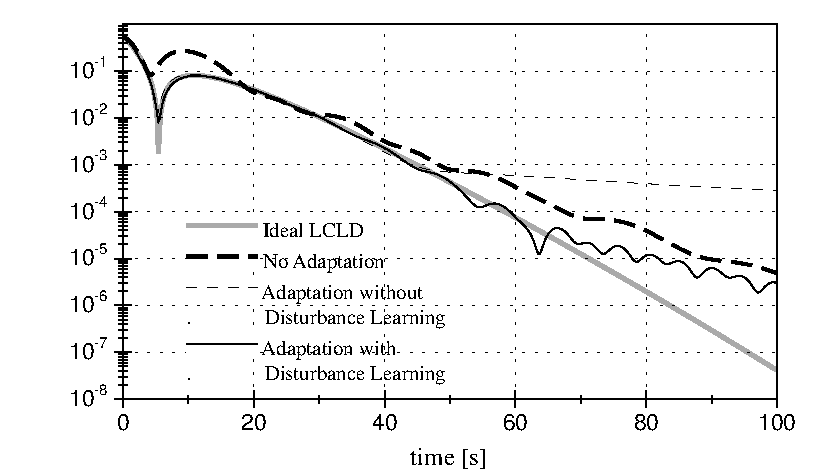
\includegraphics[]{Figures/sample}
 	\caption{Sample image}
 	\label{fig:sample}
 \end{figure}
 

 \subsubsection{Testing of a Subsection}

text here text here text here text here text here text here text here text here text here text here text here text here text here text here text here text here text here text here text here text here text here text here text here text here text here text here text here text here text here text here text here text here text here text here text here text here text here text here text here text here text here text here text here text here text here text here text here text here text 




\section{Problem Statement}
Text goes here
\begin{itemize}
	\item Explain the mathematics of the problem discussed in this paper
	\item Explain the notation, coordinate frame choices, etc.
	\item Don't develop new theories here, only show enough to warm up the reader to be able to follow the new development in the following sections.  
	\item use a figure here, if possible, to explain the general problem setup and variable name choices.  
	\item Be careful to reference where the used equations and theories are coming from.  
\end{itemize}


\section{Sections with New Work}
In these sections you discuss the new developments in detail.  Add as many section or subsections as you need.  


\section{Numerical Simulations}
Discuss any numerical simulations that you are going to use to illustrate your analytical results.  Be sure to fully explain how the simulations were achieved.  Imagine yourself reading this paper, and having to duplicate this work using only this reference.  Provide all required initial conditions, state what dynamical systems were integrated, etc.  Also, be sure to reference and discuss any result figures that you show here.



\section{Conclusion}
The conclusion you briefly summarize the paper.  Discuss what problem was solved, how it was solved, any limitations of the method.  Contrary to the introduction, you do briefly discuss the results here.  It is also ok to briefly address future research in this area.  



\section*{Acknowledgment}
Acknowledge any sponsors, or other person who are not authors, who helped create this paper.  

\bibliographystyle{aiaa}   % Number the references.
\bibliography{references}   % Use references.bib to resolve the labels.


\end{document}

